\documentclass{standalone}
\usepackage{tikz}
\usetikzlibrary{patterns, positioning}


\begin{document}
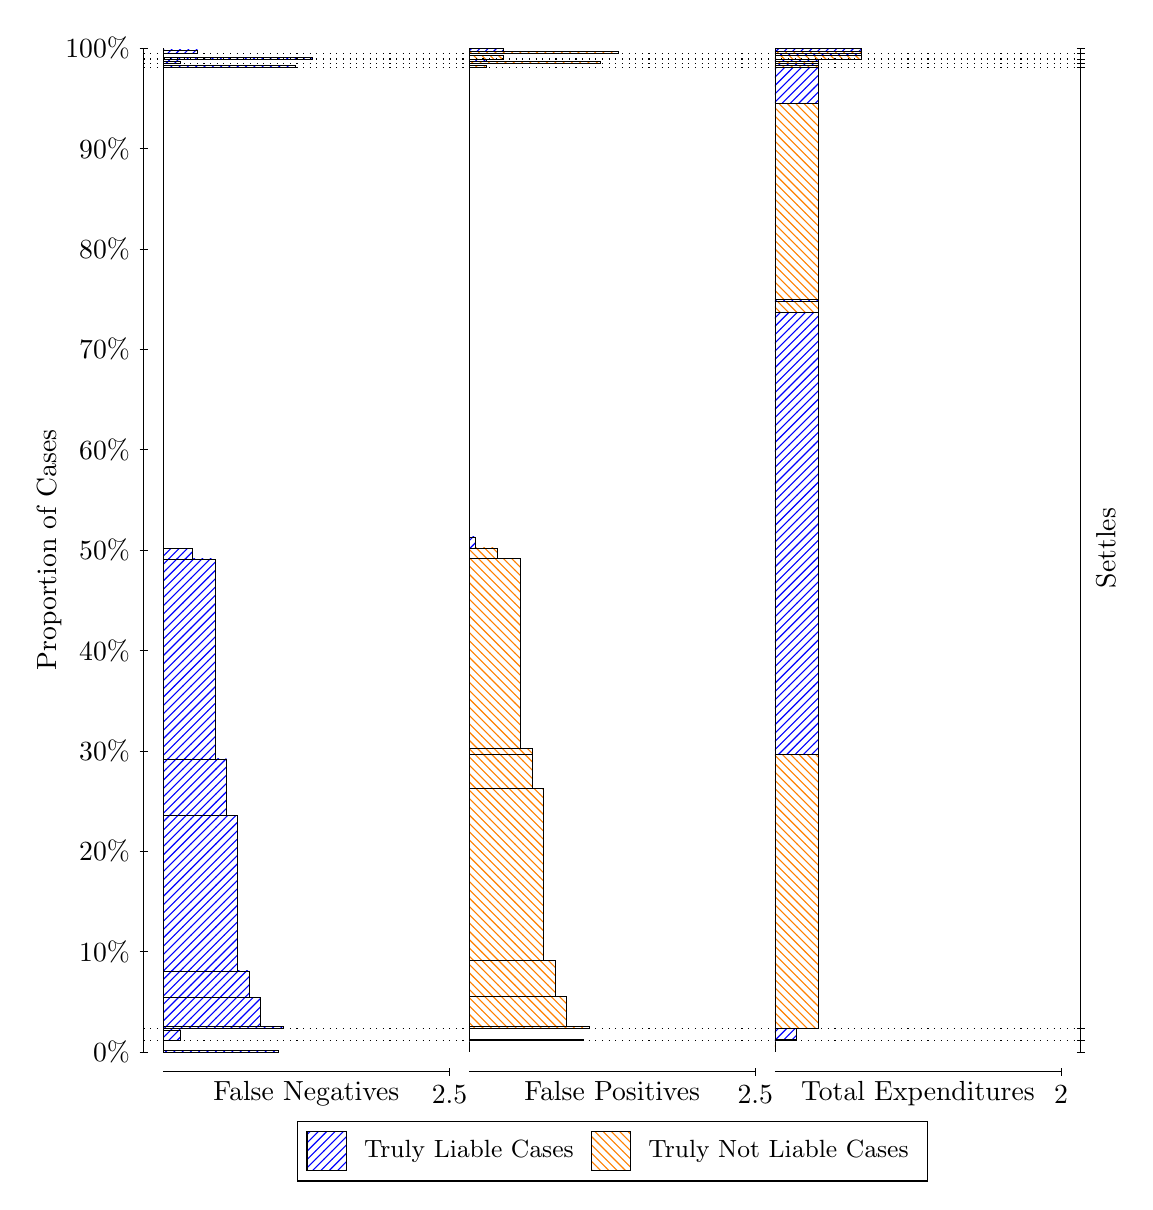
\begin{tikzpicture}
\draw[black, very thin] (1.5,1.75) -- (1.5,14.5);
\node[rotate=90, text=black, anchor=center] at (0.3, 8.125) {Proportion of Cases};
\draw[black, very thin] (1.45,1.75) -- (1.55,1.75);
\node[text=black, anchor=east] at (1.45, 1.75) {0\%};
\draw[black, very thin] (1.45,3.025) -- (1.55,3.025);
\node[text=black, anchor=east] at (1.45, 3.025) {10\%};
\draw[black, very thin] (1.45,4.3) -- (1.55,4.3);
\node[text=black, anchor=east] at (1.45, 4.3) {20\%};
\draw[black, very thin] (1.45,5.575) -- (1.55,5.575);
\node[text=black, anchor=east] at (1.45, 5.575) {30\%};
\draw[black, very thin] (1.45,6.85) -- (1.55,6.85);
\node[text=black, anchor=east] at (1.45, 6.85) {40\%};
\draw[black, very thin] (1.45,8.125) -- (1.55,8.125);
\node[text=black, anchor=east] at (1.45, 8.125) {50\%};
\draw[black, very thin] (1.45,9.4) -- (1.55,9.4);
\node[text=black, anchor=east] at (1.45, 9.4) {60\%};
\draw[black, very thin] (1.45,10.675) -- (1.55,10.675);
\node[text=black, anchor=east] at (1.45, 10.675) {70\%};
\draw[black, very thin] (1.45,11.95) -- (1.55,11.95);
\node[text=black, anchor=east] at (1.45, 11.95) {80\%};
\draw[black, very thin] (1.45,13.225) -- (1.55,13.225);
\node[text=black, anchor=east] at (1.45, 13.225) {90\%};
\draw[black, very thin] (1.45,14.5) -- (1.55,14.5);
\node[text=black, anchor=east] at (1.45, 14.5) {100\%};

\draw[black, very thin] (13.4,1.75) -- (13.4,14.5);
\draw[black, very thin] (13.35,1.75) -- (13.45,1.75);
\node[anchor=west] at (13.35, 1.75) {};
\draw[black, very thin] (13.35,1.8983) -- (13.45,1.8983);
\node[anchor=west] at (13.35, 1.8983) {};
\draw[black, very thin] (13.35,2.0465) -- (13.45,2.0465);
\node[anchor=west] at (13.35, 2.0465) {};
\draw[black, very thin] (13.35,14.255) -- (13.45,14.255);
\node[anchor=west] at (13.35, 14.255) {};
\draw[black, very thin] (13.35,14.305) -- (13.45,14.305);
\node[anchor=west] at (13.35, 14.305) {};
\draw[black, very thin] (13.35,14.36) -- (13.45,14.36);
\node[anchor=west] at (13.35, 14.36) {};
\draw[black, very thin] (13.35,14.43) -- (13.45,14.43);
\node[anchor=west] at (13.35, 14.43) {};
\draw[black, very thin] (13.35,14.5) -- (13.45,14.5);
\node[anchor=west] at (13.35, 14.5) {};

\draw[black, very thin, pattern color=blue, pattern=north east lines] (1.75,1.75) rectangle (3.2033,1.7656);
\draw[black, very thin, pattern color=orange, pattern=north west lines] (1.75,1.7656) rectangle (1.75,1.8983);
\draw[black, very thin, pattern color=blue, pattern=north east lines] (1.75,1.8983) rectangle (1.968,2.0309);
\draw[black, very thin, pattern color=orange, pattern=north west lines] (1.75,2.0309) rectangle (1.75,2.0465);
\draw[black, very thin, pattern color=blue, pattern=north east lines] (1.75,2.0465) rectangle (3.276,2.0769);
\draw[black, very thin, pattern color=blue, pattern=north east lines] (1.75,2.0769) rectangle (2.9853,2.445);
\draw[black, very thin, pattern color=blue, pattern=north east lines] (1.75,2.445) rectangle (2.84,2.7793);
\draw[black, very thin, pattern color=blue, pattern=north east lines] (1.75,2.7793) rectangle (2.6947,4.751);
\draw[black, very thin, pattern color=blue, pattern=north east lines] (1.75,4.751) rectangle (2.5493,5.4709);
\draw[black, very thin, pattern color=blue, pattern=north east lines] (1.75,5.4709) rectangle (2.404,8.0114);
\draw[black, very thin, pattern color=blue, pattern=north east lines] (1.75,8.0114) rectangle (2.1133,8.1497);
\draw[black, very thin, pattern color=orange, pattern=north west lines] (1.75,8.1497) rectangle (1.75,14.255);
\draw[black, very thin, pattern color=blue, pattern=north east lines] (1.75,14.255) rectangle (3.4213,14.276);
\draw[black, very thin, pattern color=orange, pattern=north west lines] (1.75,14.276) rectangle (1.75,14.305);
\draw[black, very thin, pattern color=blue, pattern=north east lines] (1.75,14.305) rectangle (1.968,14.338);
\draw[black, very thin, pattern color=orange, pattern=north west lines] (1.75,14.338) rectangle (1.75,14.36);
\draw[black, very thin, pattern color=blue, pattern=north east lines] (1.75,14.36) rectangle (3.6393,14.384);
\draw[black, very thin, pattern color=orange, pattern=north west lines] (1.75,14.384) rectangle (1.75,14.43);
\draw[black, very thin, pattern color=blue, pattern=north east lines] (1.75,14.43) rectangle (2.186,14.476);
\draw[black, very thin, pattern color=orange, pattern=north west lines] (1.75,14.476) rectangle (1.75,14.5);
\draw[black, very thin, pattern color=orange, pattern=north west lines] (5.6333,1.75) rectangle (5.6333,1.8827);
\draw[black, very thin, pattern color=blue, pattern=north east lines] (5.6333,1.8827) rectangle (5.6333,1.8983);
\draw[black, very thin, pattern color=orange, pattern=north west lines] (5.6333,1.8983) rectangle (7.0867,1.9139);
\draw[black, very thin, pattern color=blue, pattern=north east lines] (5.6333,1.9139) rectangle (5.6333,2.0465);
\draw[black, very thin, pattern color=orange, pattern=north west lines] (5.6333,2.0465) rectangle (7.1593,2.0769);
\draw[black, very thin, pattern color=orange, pattern=north west lines] (5.6333,2.0769) rectangle (6.8687,2.4583);
\draw[black, very thin, pattern color=orange, pattern=north west lines] (5.6333,2.4583) rectangle (6.7233,2.9149);
\draw[black, very thin, pattern color=orange, pattern=north west lines] (5.6333,2.9149) rectangle (6.578,5.0971);
\draw[black, very thin, pattern color=orange, pattern=north west lines] (5.6333,5.0971) rectangle (6.4327,5.5284);
\draw[black, very thin, pattern color=orange, pattern=north west lines] (5.6333,5.5284) rectangle (6.4327,5.6012);
\draw[black, very thin, pattern color=orange, pattern=north west lines] (5.6333,5.6012) rectangle (6.2873,8.0137);
\draw[black, very thin, pattern color=orange, pattern=north west lines] (5.6333,8.0137) rectangle (5.9967,8.152);
\draw[black, very thin, pattern color=blue, pattern=north east lines] (5.6333,8.152) rectangle (5.706,8.2903);
\draw[black, very thin, pattern color=blue, pattern=north east lines] (5.6333,8.2903) rectangle (5.6333,14.255);
\draw[black, very thin, pattern color=orange, pattern=north west lines] (5.6333,14.255) rectangle (5.8513,14.284);
\draw[black, very thin, pattern color=blue, pattern=north east lines] (5.6333,14.284) rectangle (5.6333,14.305);
\draw[black, very thin, pattern color=orange, pattern=north west lines] (5.6333,14.305) rectangle (7.3047,14.327);
\draw[black, very thin, pattern color=blue, pattern=north east lines] (5.6333,14.327) rectangle (5.8513,14.36);
\draw[black, very thin, pattern color=orange, pattern=north west lines] (5.6333,14.36) rectangle (6.0693,14.406);
\draw[black, very thin, pattern color=blue, pattern=north east lines] (5.6333,14.406) rectangle (5.6333,14.43);
\draw[black, very thin, pattern color=orange, pattern=north west lines] (5.6333,14.43) rectangle (7.5227,14.454);
\draw[black, very thin, pattern color=blue, pattern=north east lines] (5.6333,14.454) rectangle (6.0693,14.5);
\draw[black, very thin, pattern color=orange, pattern=north west lines] (9.5167,1.75) rectangle (9.5167,1.8827);
\draw[black, very thin, pattern color=blue, pattern=north east lines] (9.5167,1.8827) rectangle (9.5167,1.8983);
\draw[black, very thin, pattern color=orange, pattern=north west lines] (9.5167,1.8983) rectangle (9.7892,1.9139);
\draw[black, very thin, pattern color=blue, pattern=north east lines] (9.5167,1.9139) rectangle (9.7892,2.0465);
\draw[black, very thin, pattern color=orange, pattern=north west lines] (9.5167,2.0465) rectangle (10.062,5.5284);
\draw[black, very thin, pattern color=blue, pattern=north east lines] (9.5167,5.5284) rectangle (10.062,11.143);
\draw[black, very thin, pattern color=orange, pattern=north west lines] (9.5167,11.143) rectangle (10.062,11.282);
\draw[black, very thin, pattern color=blue, pattern=north east lines] (9.5167,11.282) rectangle (10.062,11.312);
\draw[black, very thin, pattern color=orange, pattern=north west lines] (9.5167,11.312) rectangle (10.062,13.797);
\draw[black, very thin, pattern color=blue, pattern=north east lines] (9.5167,13.797) rectangle (10.062,14.255);
\draw[black, very thin, pattern color=orange, pattern=north west lines] (9.5167,14.255) rectangle (10.062,14.284);
\draw[black, very thin, pattern color=blue, pattern=north east lines] (9.5167,14.284) rectangle (10.062,14.305);
\draw[black, very thin, pattern color=orange, pattern=north west lines] (9.5167,14.305) rectangle (10.062,14.327);
\draw[black, very thin, pattern color=blue, pattern=north east lines] (9.5167,14.327) rectangle (10.062,14.36);
\draw[black, very thin, pattern color=orange, pattern=north west lines] (9.5167,14.36) rectangle (10.607,14.406);
\draw[black, very thin, pattern color=blue, pattern=north east lines] (9.5167,14.406) rectangle (10.607,14.43);
\draw[black, very thin, pattern color=orange, pattern=north west lines] (9.5167,14.43) rectangle (10.607,14.454);
\draw[black, very thin, pattern color=blue, pattern=north east lines] (9.5167,14.454) rectangle (10.607,14.5);
\draw[black, dotted] (1.5,1.8983) -- (13.4,1.8983);
\draw[black, dotted] (1.5,2.0465) -- (13.4,2.0465);
\draw[black, dotted] (1.5,14.255) -- (13.4,14.255);
\draw[black, dotted] (1.5,14.305) -- (13.4,14.305);
\draw[black, dotted] (1.5,14.36) -- (13.4,14.36);
\draw[black, dotted] (1.5,14.43) -- (13.4,14.43);
\draw[black, very thin] (1.75,1.5) -- (5.3833,1.5);
\node[text=black, anchor=north] at (3.5667, 1.5) {False Negatives};
\draw[black, very thin] (5.3833,1.45) -- (5.3833,1.55);
\node[text=black, anchor=north] at (5.3833, 1.45) {2.5};

\draw[black, very thin] (5.6333,1.5) -- (9.2667,1.5);
\node[text=black, anchor=north] at (7.45, 1.5) {False Positives};
\draw[black, very thin] (9.2667,1.45) -- (9.2667,1.55);
\node[text=black, anchor=north] at (9.2667, 1.45) {2.5};

\draw[black, very thin] (9.5167,1.5) -- (13.15,1.5);
\node[text=black, anchor=north] at (11.333, 1.5) {Total Expenditures};
\draw[black, very thin] (13.15,1.45) -- (13.15,1.55);
\node[text=black, anchor=north] at (13.15, 1.45) {2};



\node[text=black, centered, rotate=90] at (13.72, 8.1508) {Settles};





\draw (7.449999999999999,1.5) node[draw=none] (baseCoordinate) {};
\begin{scope}[align=center]
        \matrix[scale=0.5, draw=black, below=0.5cm of baseCoordinate, nodes={draw}, column sep=0.1cm]{
            \node[rectangle, draw, minimum width=0.5cm, minimum height=0.5cm, pattern color=blue, pattern=north east lines] {}; &
            \node[draw=none, font=\small, text=black] (B) {Truly Liable Cases}; &
            \node[rectangle, draw, minimum width=0.5cm, minimum height=0.5cm, pattern color=orange, pattern=north west lines] {}; &
            \node[draw=none, font=\small, text=black] (B) {Truly Not Liable Cases}; \\
            };
\end{scope}

\end{tikzpicture}
\end{document}